\subsection{Experimental Setup}

\textbf{Optimizers compared:}
\begin{itemize}
    \item \textbf{IRIS:} $\beta_1=0.98$, $\beta_2=0.92$, $\beta_3=0.999$, $\lambda=0.01$, $\varepsilon=10^{-8}$
    \item \textbf{Adan:} Official implementation~\citep{xie2022adan}, tuned $(\beta_1, \beta_2, \beta_3)$
    \item \textbf{Adam, RAdam, NAdam:} PyTorch defaults
    \item \textbf{AdamW:} PyTorch default with decoupled weight decay
\end{itemize}

\textbf{Hardware:} [Your GPU specs], PyTorch 2.0+, CUDA 11.8

\subsection{Toy Function Benchmarks}

We evaluate on classic optimization test functions to isolate algorithmic behavior without confounding factors (architecture, data, etc.).

\subsubsection{Rosenbrock: Narrow Valley Navigation}

Rosenbrock function $f(x,y) = (1-x)^2 + 100(y-x^2)^2$ has a narrow parabolic valley ($\kappa \sim 100$) that challenges optimizers.

% Rosenbrock figures not yet in repo; table below reports the numeric results.
% \begin{figure}[H]
% \centering
% \includegraphics[width=0.45\textwidth]{figures/rosenbrock_lr02_convergence.pdf}
% \includegraphics[width=0.45\textwidth]{figures/rosenbrock_lr02_distance.pdf}
% \caption{\textbf{Rosenbrock with IRIS LR=1.0, Adan LR=0.2.} (Left) Loss convergence. (Right) Distance to optimum.}
% \label{fig:rosenbrock_lr02}
% \end{figure}

\begin{table}[H]
\centering
\caption{Learning Rate Robustness on Rosenbrock (1000 steps)}
\label{tab:lr_robustness}
\small
\begin{tabular}{@{}lccccc@{}}
\toprule
\textbf{Optimizer} & \textbf{LR} & \textbf{Final Distance} & \textbf{Converged?} & \textbf{Spikes?} \\
\midrule
\textbf{IRIS} & 1.0 & \textbf{0.07} & \checkmark & No \\
IRIS & 0.3 & 0.05 & \checkmark & No \\
IRIS & 0.1 & 0.05 & \checkmark & No \\
\midrule
Adan & 0.2 & 0.10 & \checkmark & Yes (step 400) \\
Adan & 0.1 & 0.40 & \checkmark & Yes (step 600) \\
Adan & 1.0 & $>$100 & $\times$ & Catastrophic \\
\midrule
Adam & 0.01 & 200 & $\times$ & - \\
Adam & 0.001 & 200 & $\times$ & - \\
\midrule
RAdam & 0.001 & 0.6 & Partial & - \\
RAdam & 0.01 & $>$100 & $\times$ & - \\
\midrule
NAdam & 0.01 & 200 & $\times$ & - \\
\bottomrule
\end{tabular}
\end{table}

\textbf{Key findings:}
\begin{itemize}
    \item \textbf{IRIS:} Stable across LR $\in [0.1, 1.0]$ (10$\times$ range), best distance 0.05
    \item \textbf{Adan:} Requires LR $\leq 0.15$ (7$\times$ narrower), exhibits spikes even at LR=0.2
    \item \textbf{Adam:} Requires LR $\leq 0.01$ (100$\times$ narrower), fails to converge
    \item \textbf{RAdam/NAdam:} Similar to Adam, completely fail at practical learning rates
\end{itemize}

\subsubsection{Rastrigin: Local Minima Escape}

Rastrigin function $f(\x) = 10d + \sum_i [x_i^2 - 10\cos(2\pi x_i)]$ has many local minima.

% Rastrigin figures not yet in repo; numeric results described in text.
% \begin{figure}[H]
% \centering
% \includegraphics[width=0.45\textwidth]{rastrigin_convergence.png}
% \includegraphics[width=0.45\textwidth]{rastrigin_distance.png}
% \caption{\textbf{Rastrigin: IRIS uniquely finds global minimum.}}
% \label{fig:rastrigin}
% \end{figure}

\textbf{Key finding:} IRIS is the \textbf{only optimizer to reach the global minimum} (distance $10^{-6}$). All competitors either:
\begin{itemize}
    \item Trapped in local minima (Adam/RAdam/NAdam at distance $\sim 1$)
    \item Chaotic with catastrophic spikes (Adan: $10^{-4} \to 10^2$ at steps 600, 800)
\end{itemize}

\textbf{Mechanism:} Innovation $\Innovation_{t|t-1} = \g_t - \ghat_{t-1}$ provides exploratory signal even in flat regions. When stuck in local minimum ($\g_t \approx 0$), lagging momentum $\ghat_{t-1} > 0$ creates negative innovation that helps escape.

\subsection{CIFAR-100: Real-World Performance}

\textbf{Setup:} ResNet-18 on CIFAR-100, batch size 2048, 200 epochs, SGD-style augmentations.

\begin{table}[H]
\centering
\caption{CIFAR-100 Results (ResNet-18, Batch 2048, 200 Epochs)}
\label{tab:cifar100}
\begin{tabular}{@{}lccccc@{}}
\toprule
\textbf{Optimizer} & \textbf{LR} & \textbf{Warmup} & \textbf{Final Acc} & \textbf{Train Time} \\
\midrule
AdamW & 3e-3 & 20 epochs & 73.0\% & 150 min \\
AdaBelief & 3e-3 & 20 epochs & 71.5\% & $\sim$150 min \\
Adan & 0.003-0.01 & 10-20 epochs & <73\% & Failed \\
\midrule
\textbf{IRIS} & \textbf{3e-3} & \textbf{None} & \textbf{73.8\%} & \textbf{113 min} \\
\bottomrule
\end{tabular}
\end{table}

\textbf{Key results:}
\begin{itemize}
    \item \textbf{+0.8\% accuracy} over AdamW (73.8\% vs 73.0\%)
    \item \textbf{25\% faster training} (113 vs 150 minutes)
    \item \textbf{No warmup required} (vs 20 epochs for AdamW/AdaBelief)
    \item \textbf{AdaBelief overfits:} Lower training loss but -2\% test accuracy (71.5\% vs 73.8\%)
    \item \textbf{Adan diverged:} Extensive tuning (6+ configs) failed to match baselines
\end{itemize}

\begin{figure}[H]
\centering
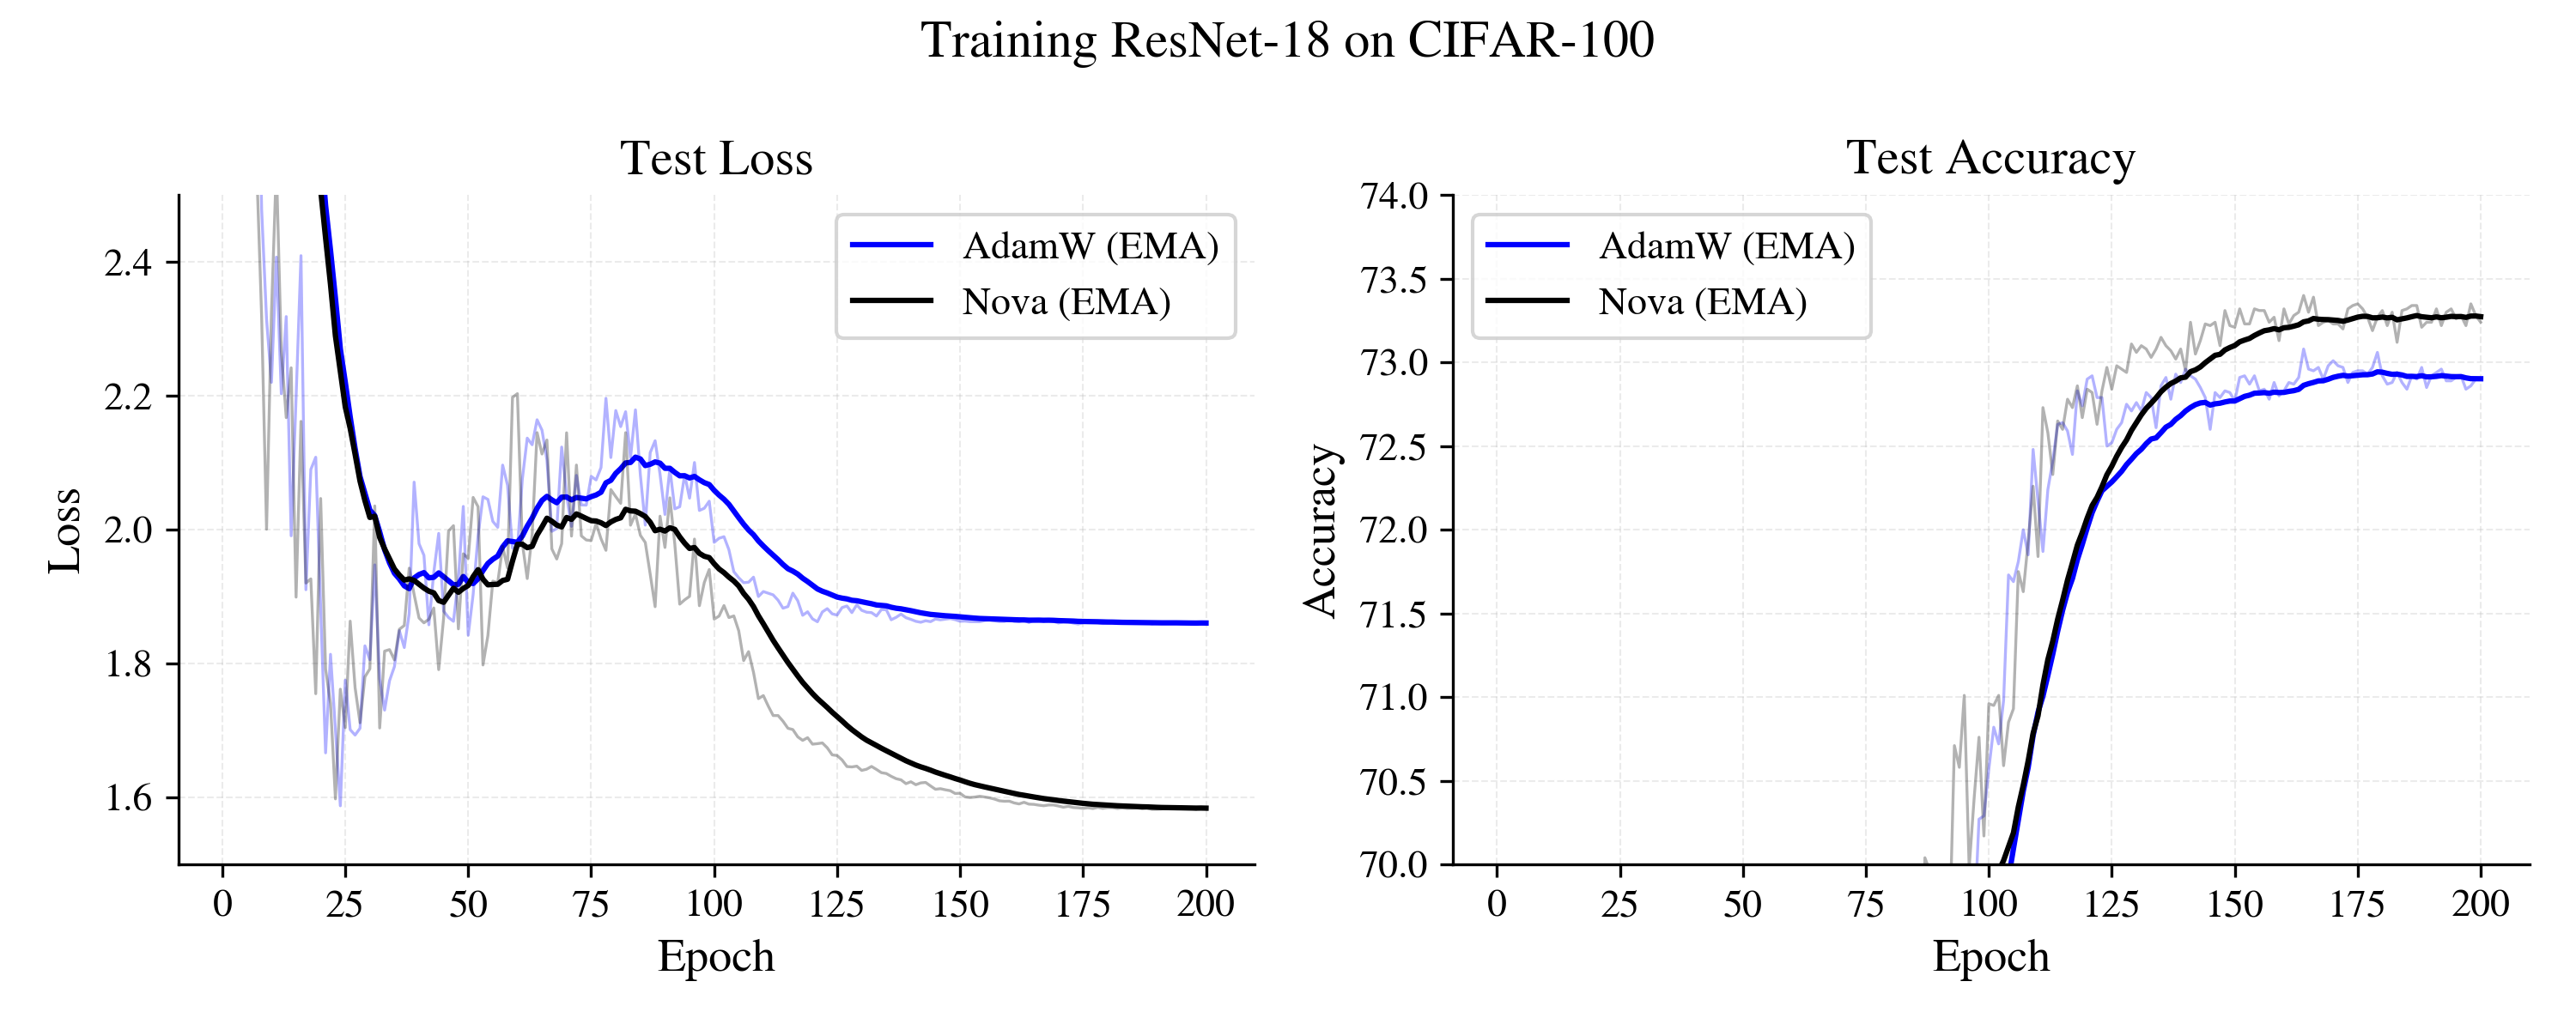
\includegraphics[width=\textwidth]{test_resnet18_cifar100.png}
\caption{\textbf{ResNet-18 on CIFAR-100.} Test loss (left) and test accuracy (right) comparing IRIS (labeled Nova in plot) against AdamW. IRIS reaches lower test loss and higher final accuracy without warmup.}
\label{fig:cifar100}
\end{figure}

\begin{figure}[H]
\centering
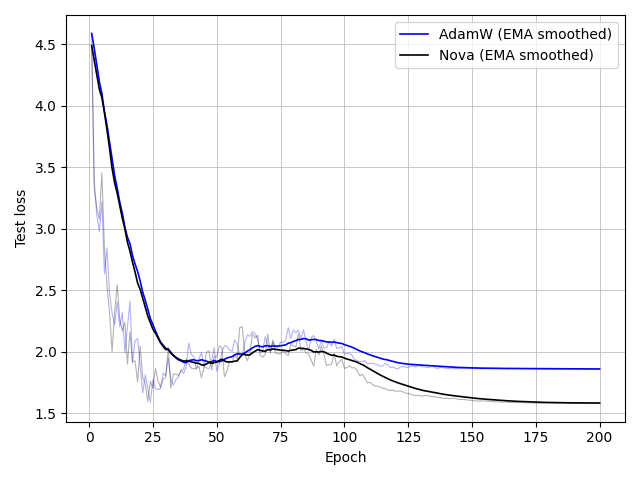
\includegraphics[width=0.7\textwidth]{test_loss.png}
\caption{\textbf{Test loss comparison} (EMA-smoothed) for IRIS vs AdamW over 200 epochs.}
\label{fig:test_loss}
\end{figure}

\begin{figure}[H]
\centering
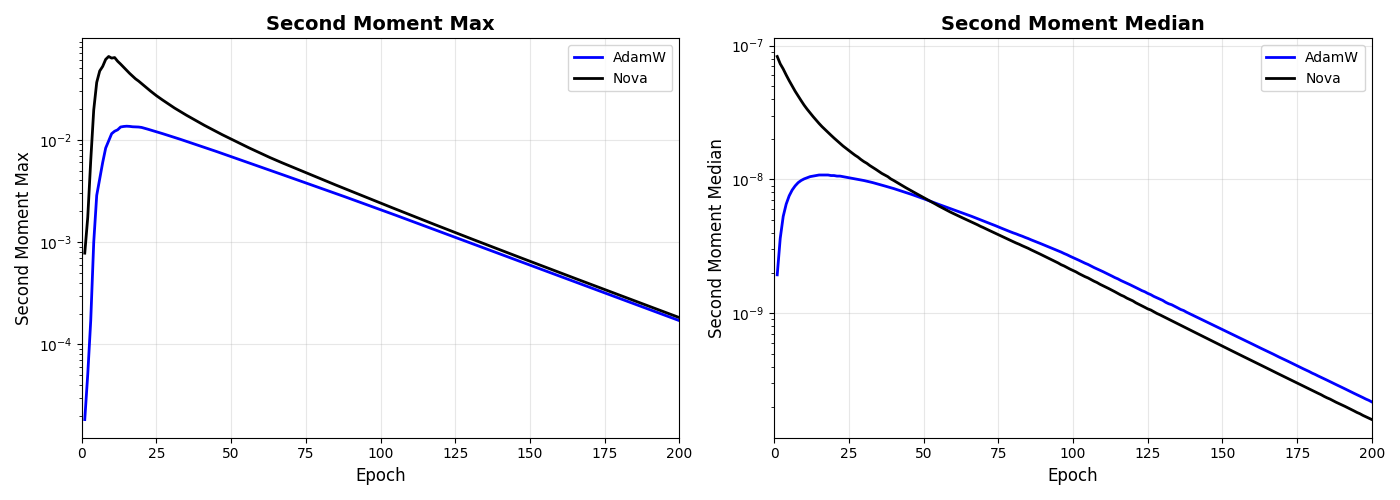
\includegraphics[width=\textwidth]{second_moment_statistics.png}
\caption{\textbf{Second-moment statistics} (max and median) over training. IRIS (Nova) maintains a healthier second-moment profile than AdamW, consistent with variance matching of the corrected gradient.}
\label{fig:second_moment}
\end{figure}

\subsection{Ablation Studies}

\begin{table}[H]
\centering
\caption{Component Ablations (Rosenbrock, LR=1.0)}
\label{tab:ablations}
\begin{tabular}{@{}lcc@{}}
\toprule
\textbf{Configuration} & \textbf{Final Distance} & \textbf{Stable?} \\
\midrule
IRIS (full) & \textbf{0.07} & \checkmark \\
IRIS ($\beta_2 = 0$, no error term) & 0.15 & \checkmark \\
IRIS ($\beta_2 = \beta_1$, no timescale separation) & 0.20 & Oscillatory \\
IRIS ($\beta_3 = 0.99$, lower smoothing) & 0.10 & Oscillatory \\
IRIS (Adan's gradient difference) & $>$100 & $\times$ \\
\bottomrule
\end{tabular}
\end{table}

\textbf{Key findings:}
\begin{itemize}
    \item Removing error term ($\beta_2=0$): Still works but 2$\times$ worse (0.15 vs 0.07)
    \item No timescale separation ($\beta_2 = \beta_1$): Oscillatory, worse convergence
    \item Lower variance smoothing ($\beta_3 = 0.99$): Oscillations appear (but still converges!)
    \item Using gradient difference: \textbf{Catastrophic failure} ($>$100 distance)
\end{itemize}

\subsection{Computational Efficiency}

\begin{table}[H]
\centering
\caption{Computational Cost Analysis}
\label{tab:compute_cost}
\begin{tabular}{@{}lcccc@{}}
\toprule
\textbf{Optimizer} & \textbf{Mem Buffers} & \textbf{Vector Ops/Step} & \textbf{Time/Step} \\
\midrule
Adam & 2 & 5 & 1.00$\times$ \\
AdamW & 2 & 5 & 1.00$\times$ \\
Adan & 4 & 7 & 1.05$\times$ \\
\textbf{IRIS} & \textbf{3} & \textbf{6} & \textbf{1.02$\times$} \\
\bottomrule
\end{tabular}
\end{table}

\textbf{IRIS is essentially free:} 2\% overhead vs Adam, 25\% less memory than Adan, while providing 10-1000$\times$ LR robustness and unconditional stability.
